\documentclass[11pt,ignorenonframetext,]{beamer}
\setbeamertemplate{caption}[numbered]
\setbeamertemplate{caption label separator}{: }
\setbeamercolor{caption name}{fg=normal text.fg}
\beamertemplatenavigationsymbolsempty
\usepackage{lmodern}
\usepackage{amssymb,amsmath}
\usepackage{ifxetex,ifluatex}
\usepackage{fixltx2e} % provides \textsubscript
\ifnum 0\ifxetex 1\fi\ifluatex 1\fi=0 % if pdftex
  \usepackage[T1]{fontenc}
  \usepackage[utf8]{inputenc}
\else % if luatex or xelatex
  \ifxetex
    \usepackage{mathspec}
  \else
    \usepackage{fontspec}
  \fi
  \defaultfontfeatures{Ligatures=TeX,Scale=MatchLowercase}
\fi
% use upquote if available, for straight quotes in verbatim environments
\IfFileExists{upquote.sty}{\usepackage{upquote}}{}
% use microtype if available
\IfFileExists{microtype.sty}{%
\usepackage{microtype}
\UseMicrotypeSet[protrusion]{basicmath} % disable protrusion for tt fonts
}{}
\newif\ifbibliography
\hypersetup{
            pdftitle={Causal inference and experimental methods},
            pdfauthor={Macartan Humphreys},
            pdfborder={0 0 0},
            breaklinks=true}
\urlstyle{same}  % don't use monospace font for urls
\usepackage{color}
\usepackage{fancyvrb}
\newcommand{\VerbBar}{|}
\newcommand{\VERB}{\Verb[commandchars=\\\{\}]}
\DefineVerbatimEnvironment{Highlighting}{Verbatim}{commandchars=\\\{\}}
% Add ',fontsize=\small' for more characters per line
\usepackage{framed}
\definecolor{shadecolor}{RGB}{248,248,248}
\newenvironment{Shaded}{\begin{snugshade}}{\end{snugshade}}
\newcommand{\KeywordTok}[1]{\textcolor[rgb]{0.13,0.29,0.53}{\textbf{#1}}}
\newcommand{\DataTypeTok}[1]{\textcolor[rgb]{0.13,0.29,0.53}{#1}}
\newcommand{\DecValTok}[1]{\textcolor[rgb]{0.00,0.00,0.81}{#1}}
\newcommand{\BaseNTok}[1]{\textcolor[rgb]{0.00,0.00,0.81}{#1}}
\newcommand{\FloatTok}[1]{\textcolor[rgb]{0.00,0.00,0.81}{#1}}
\newcommand{\ConstantTok}[1]{\textcolor[rgb]{0.00,0.00,0.00}{#1}}
\newcommand{\CharTok}[1]{\textcolor[rgb]{0.31,0.60,0.02}{#1}}
\newcommand{\SpecialCharTok}[1]{\textcolor[rgb]{0.00,0.00,0.00}{#1}}
\newcommand{\StringTok}[1]{\textcolor[rgb]{0.31,0.60,0.02}{#1}}
\newcommand{\VerbatimStringTok}[1]{\textcolor[rgb]{0.31,0.60,0.02}{#1}}
\newcommand{\SpecialStringTok}[1]{\textcolor[rgb]{0.31,0.60,0.02}{#1}}
\newcommand{\ImportTok}[1]{#1}
\newcommand{\CommentTok}[1]{\textcolor[rgb]{0.56,0.35,0.01}{\textit{#1}}}
\newcommand{\DocumentationTok}[1]{\textcolor[rgb]{0.56,0.35,0.01}{\textbf{\textit{#1}}}}
\newcommand{\AnnotationTok}[1]{\textcolor[rgb]{0.56,0.35,0.01}{\textbf{\textit{#1}}}}
\newcommand{\CommentVarTok}[1]{\textcolor[rgb]{0.56,0.35,0.01}{\textbf{\textit{#1}}}}
\newcommand{\OtherTok}[1]{\textcolor[rgb]{0.56,0.35,0.01}{#1}}
\newcommand{\FunctionTok}[1]{\textcolor[rgb]{0.00,0.00,0.00}{#1}}
\newcommand{\VariableTok}[1]{\textcolor[rgb]{0.00,0.00,0.00}{#1}}
\newcommand{\ControlFlowTok}[1]{\textcolor[rgb]{0.13,0.29,0.53}{\textbf{#1}}}
\newcommand{\OperatorTok}[1]{\textcolor[rgb]{0.81,0.36,0.00}{\textbf{#1}}}
\newcommand{\BuiltInTok}[1]{#1}
\newcommand{\ExtensionTok}[1]{#1}
\newcommand{\PreprocessorTok}[1]{\textcolor[rgb]{0.56,0.35,0.01}{\textit{#1}}}
\newcommand{\AttributeTok}[1]{\textcolor[rgb]{0.77,0.63,0.00}{#1}}
\newcommand{\RegionMarkerTok}[1]{#1}
\newcommand{\InformationTok}[1]{\textcolor[rgb]{0.56,0.35,0.01}{\textbf{\textit{#1}}}}
\newcommand{\WarningTok}[1]{\textcolor[rgb]{0.56,0.35,0.01}{\textbf{\textit{#1}}}}
\newcommand{\AlertTok}[1]{\textcolor[rgb]{0.94,0.16,0.16}{#1}}
\newcommand{\ErrorTok}[1]{\textcolor[rgb]{0.64,0.00,0.00}{\textbf{#1}}}
\newcommand{\NormalTok}[1]{#1}
\usepackage{graphicx,grffile}
\makeatletter
\def\maxwidth{\ifdim\Gin@nat@width>\linewidth\linewidth\else\Gin@nat@width\fi}
\def\maxheight{\ifdim\Gin@nat@height>\textheight0.8\textheight\else\Gin@nat@height\fi}
\makeatother
% Scale images if necessary, so that they will not overflow the page
% margins by default, and it is still possible to overwrite the defaults
% using explicit options in \includegraphics[width, height, ...]{}
\setkeys{Gin}{width=\maxwidth,height=\maxheight,keepaspectratio}

% Prevent slide breaks in the middle of a paragraph:
\widowpenalties 1 10000
\raggedbottom

\AtBeginPart{
  \let\insertpartnumber\relax
  \let\partname\relax
  \frame{\partpage}
}
\AtBeginSection{
  \ifbibliography
  \else
    \let\insertsectionnumber\relax
    \let\sectionname\relax
    \frame{\sectionpage}
  \fi
}
\AtBeginSubsection{
  \let\insertsubsectionnumber\relax
  \let\subsectionname\relax
  \frame{\subsectionpage}
}

\setlength{\parindent}{0pt}
\setlength{\parskip}{6pt plus 2pt minus 1pt}
\setlength{\emergencystretch}{3em}  % prevent overfull lines
\providecommand{\tightlist}{%
  \setlength{\itemsep}{0pt}\setlength{\parskip}{0pt}}
\setcounter{secnumdepth}{5}
\setbeamertemplate{navigation symbols}{}

\title{Causal inference and experimental methods}
\author{Macartan Humphreys}
\date{Feb 2017}

\begin{document}
\frame{\titlepage}

\begin{frame}{Take home ideas}

\begin{itemize}
\item
  A causal claim is a claim about what did not happen.
\item
  Random assignment to treatment is random sampling from alternative
  universes.
\item
  You have to have an estimand. You should be able to describe this in
  terms of \textbf{potential outcomes}.
\end{itemize}

\end{frame}

\begin{frame}{Motivation}

The \textit{intervention} based motivation for understanding causal
effects:

\begin{itemize}
    \item  We want to know if a particular  intervention (like aid) caused a particular outcome (like reduced corruption). 
    \item  We need to know:
\begin{enumerate}
    \item What happened?
    \item What would the outcome have been if there were no intervention?
\end{enumerate}

    \item  The problem
\begin{enumerate}
    \item \dots this is hard
    \item \dots this is impossible
\end{enumerate}

The problem in 2 is that you need to know what would have happened if things were different. You need information on a \textbf{counterfactual}
\end{itemize}

\end{frame}

\begin{frame}{Notation}

We will use:

\begin{itemize}
\item
  \(Y\) to denote an outcome (the dependent variable, the left hand side
  variables, the endogeneous variables)
\item
  \(X\) to denote a cause (the independent variable, the driver, the
  right hand side variables, the exogeneous variables)
\item
  \(X_1, X_2, \dots\) for particular causes
\end{itemize}

Different research projects:

\begin{itemize}
\tightlist
\item
  \(? \rightarrow Y\): What causes \(Y\)?
\item
  \(X \rightarrow ?\): What does \(X\) do?
\item
  \(X \rightarrow Y ?\): Does \(X\) cause \(Y\)?
\item
  \(? \rightarrow ? ?\): What's up?
\end{itemize}

Know your \(X\) and your \(Y\).

\end{frame}

\section{The Potential Outcomes
Framework}\label{the-potential-outcomes-framework}

\begin{frame}{Potential Outcomes: Simple case}

\begin{itemize}
    \item For each unit we assume that there are two \textbf{post-treatment} outcomes: $Y_i(1)$ and $Y_i(0)$. 
    \item eg $Y(1)$ is the outcome that \textbf{would} obtain \textit{if} the unit received the treatment. 
    \item  The \textbf{causal effect }of Treatment (relative to Control) is:
    $$ \tau_i = Y_i(1) - Y_i(0)$$
    \item Note: 
    
\begin{itemize}
    \item the causal effect is defined at the \textit{individual level}. 
    \item there is no ``data generating process'' or functional form 
    \item the causal effect is defined relative to something else and so a counterfactual must be conceivable (did Germany cause the second world war?)
    \item are there any substantive assumptions made here so far?
\end{itemize}
\end{itemize}

\end{frame}

\begin{frame}{Causal claims: What is seen?}

\begin{itemize}
    \item We have talked about what's potential, now what {do} we \textit{observe}? 
    \item Say $Z_i$ indicates whether the unit $i$ is assigned to treatment $(Z_i=1)$ or not $(Z_i=0)$. It describes the treatment process. Then what we observe is:
    $$ Y_i = Z_iY_i(1) + (1-Z_i)Y_i(0) $$

\item Say $Z$ is a random variable, then this is a sort of data generating process. BUT the key things to note is   
\begin{itemize}
    \item   $Y_i$ is random but the randomness comes from $Z_i$ --- the potential outcomes, $Y_i(1)$, $Y_i(0)$ are fixed 
    \item Compare this to a regression approach in which $Y$ is random but the $X$'s are fixed. eg:
    $$ Y \sim N(\beta X, \sigma^2) \text{ or }  Y=\alpha+\beta X+\epsilon, \epsilon\sim N(0, \sigma^2) $$
\end{itemize}
\end{itemize}

\end{frame}

\section{Implications of the counterfactual
definition}\label{implications-of-the-counterfactual-definition}

\begin{frame}{Statements about what did not happen}

\textbf{Inference}: We define causes in terms of things that did not
happen. This puts \textbf{inference} front and center.

Compare this to a \textbf{structural approach}. In a structural approach
we assume a data generating process in which outcome \(Y\) is a function
of \(X\). \[y = f_Y(x, u_Y), u_Y\sim p_Y\]

Compared to: \[ Y_i = Z_iY_i(1) + (1-Z_i)Y_i(0) \]

\begin{itemize}
\tightlist
\item
  Here knowing the effect of \(X\) on \(Y\) means knowing the functional
  form \(f_Y\) and knowing background conditions, \(u_Y\).
\item
  It does not require forming beliefs about what did not happen (the
  counterfactual claims are now buried inside \(f_Y\))
\end{itemize}

\end{frame}

\begin{frame}{Structural approach}

\textbf{Illustration}: Say that cellphones turn on if and only if they
are \textbf{intact} and have a \textbf{charged battery}.

\emph{Question}: Does providing a charged battery cause cellphones to
turn on?

\begin{itemize}
\tightlist
\item
  In the \textbf{potential outcomes} framework this requires making
  guesses from the data about how cellphones work with and without
  batteries. It is not a measure problem, but an \emph{inference}
  problem.
\item
  For the \textbf{structural approach} this figuring out whether
  cellphones are intact. It is masurement problem (conditional on the
  model).
\end{itemize}

\end{frame}

\begin{frame}{Causal claims: Transitivity and connectedness}

Now that we have a concept of causal effects available, let's answer two
\textbf{questions}:

\begin{itemize}
        \item If for a given unit $A$ causes $B$ and $B$ causes $C$, does that mean that $A$ causes $C$? 
        
        \color{white}\small A boulder is flying down a mountain. You duck. This saves your life.  
            
            So the boulder caused the ducking and the ducking caused you to survive. So: \textit{did the boulder cause you to survive?} 
        \color{black}
        \item Say $A$ causes $B$ --- does that mean that there is a spatiotemporally continuous sequence of causal intermediates? 
        
        \color{white}\small Person A is planning some action Y; Person B sets out to stop them; person X intervenes and prevents person B from stopping person A. In this case Person A may complete their action, producing Y, without any knowledge that B and X even exist; in particular B and X need not be anywhere close to the action. So: \textit{ did X cause Y}? 
\end{itemize}

\end{frame}

\begin{frame}{Causal claims: Transitivity and connectedness}

Now that we have a concept of causal effects available, let's answer two
\textbf{questions}:

\begin{itemize}
        \item If for a given unit $A$ causes $B$ and $B$ causes $C$, does that mean that $A$ causes $C$? 
        
        \color{red}\small A boulder is flying down a mountain. You duck. This saves your life.  
            
            So the boulder caused the ducking and the ducking caused you to survive. So: \textit{did the boulder cause you to survive?} 
        \color{black}
        \item Say $A$ causes $B$ --- does that mean that there is a spatiotemporally continuous sequence of causal intermediates? 
        
        \color{red}\small Person A is planning some action Y; Person B sets out to stop them; person X intervenes and prevents person B from stopping person A. In this case Person A may complete their action, producing Y, without any knowledge that B and X even exist; in particular B and X need not be anywhere close to the action. So: \textit{ did X cause Y}? 
\end{itemize}

\end{frame}

\begin{frame}{Causal claims: Contribution or attribution?}

The counterfactual model is all about contribution, not attribution,
except in a very conditional sense.

\begin{itemize}
\tightlist
\item
  Focus is on non-rival contributions
\item
  Not: what caused \(Y\) but \textbf{what is the effect of \(X\)}?
\item
  At most it provides a conditional account
\end{itemize}

Consider at outcome \(Y\) that might depend on two causes \(X_1\) and
\(X_2\): \[Y(0,0) = 0\] \[Y(1,0) = 0\] \[Y(0,1) = 0\] \[Y(1,1) = 1\]

What caused \(Y\)? Which cause was most important?

\end{frame}

\begin{frame}{Causal claims: Contribution or attribution?}

The counterfactual model is all about contribution, not attribution,
except in a very conditional sense.

\begin{itemize}
\item
  Focus is on non-rival contributions
\item
  Not: what caused \(Y\) but what is the effect of \(X\)?
\item
  At most it provides a conditional account
\item
  This is problem for research programs that define ``explanation'' in
  terms of figuring out the things that cause Y
\item
  Real difficulties conceptualizing what it means to say one cause is
  more important than another cause. What does that mean?
\end{itemize}

\end{frame}

\begin{frame}{Causal claims: Contribution or attribution?}

The counterfactual model is all about contribution, not attribution,
except in a very conditional sense.

\begin{itemize}
\item
  Focus is on non-rival contributions
\item
  Not: what caused \(Y\) but what is the effect of \(X\)?
\item
  At most it provides a conditional account
\item
  \emph{Erdogan's increasing authoritarianism was the most important
  reason for the attempted coup}

  \begin{itemize}
  \tightlist
  \item
    More important than Turkey's history of coups?
  \item
    What does that mean?
  \end{itemize}
\end{itemize}

\end{frame}

\begin{frame}{The difference between an \emph{actual} cause a
\emph{counterfactual} cause}

\begin{itemize}
\tightlist
\item
  Susie and Billy throw rocks at a bottle
\item
  Both are great aims and, if they were the only ones throwing, would
  certainly hit the bottl.e
\item
  Susie is a faster throw however and her rock hits the bottle first.
\item
  Billy's throw is a little slower and flys past the now broken bottle.
\end{itemize}

\textbf{Question}: Which stone broke the bottle?

\end{frame}

\begin{frame}{The difference between an \emph{actual} cause and a
\emph{counterfactual} cause}

\begin{itemize}
\tightlist
\item
  Susie and Billy throw rocks at a bottle
\item
  Both are great aims and, if they were the only ones throwing, would
  certainly hit the bottl.e
\item
  Susie is a faster throw however and her rock hits the bottle first.
\item
  Billy's throw is a little slower and flys past the now broken bottle.
\end{itemize}

\textbf{Question}: From a counterfactual perspective \emph{neither}
broke the bottle since the bottle would have broken in the absence of
any single throw. Yet it seems obvious that Susie's throw actually broke
the bottle. (To think about: what does ``actually'' caused actually
mean?)

\end{frame}

\begin{frame}{Causal claims: No causation without manipulation}

\begin{itemize}
\tightlist
\item
  Some seemingly causal claims not admissible.
\item
  To get the definition off the ground, \textbf{manipulation must be
  imaginable} (whether practical or not)
\item
  This renders thinking about effects of race and gender difficult
\item
  What does it mean to say that Aunt Pat voted for Brexit because she is
  old?
\end{itemize}

\end{frame}

\begin{frame}{Causal claims: No causation without manipulation}

\begin{itemize}
\tightlist
\item
  Some seemingly causal claims not admissible.
\item
  To get the definition of hte ground, \textbf{manipulation must be
  imaginable} (whether practical or not)
\item
  This renders thinking about effects of race and gender difficult
\item
  \textbf{Compare}: What does it mean to say that Southern counties
  voted for Brexit because they have many old people?
\end{itemize}

\end{frame}

\begin{frame}{Causal claims: Causal claims are everywhere}

Which of these statements involve causal claims:

\begin{itemize}
\tightlist
\item
  Jack exploited Jill
\item
  It's Jill's fault that bucket fell
\item
  Jack is the most obstructionist member of Congress
\item
  Melania Trump stole from Michelle Obama's speech
\end{itemize}

So:

\begin{itemize}
\tightlist
\item
  Policymakers and activists need causal claims
\end{itemize}

\end{frame}

\section{The Fundamental Problem and a
Solution}\label{the-fundamental-problem-and-a-solution}

\begin{frame}{Causal claims: The estimand and the rub}

\begin{itemize}
    \item  The causal effect of Treatment (relative to Control) is:
    $$ \tau_i = Y_i(1) - Y_i(0)$$
    \item This is what we want to estimate 
    \item BUT: We never can observe both $Y_i(1)$ and $Y_i(0)$!
    \item This is the \textbf{fundamental problem} (Holland)
\end{itemize}

\end{frame}

\begin{frame}{Causal claims: The rub and the solution}

\begin{itemize} \small
    \item  Now for some magic. We really want to estimate:  $$ \tau_i = Y_i(1) - Y_i(0)$$
    \item BUT: We never can observe both $Y_i(1)$ and $Y_i(0)$
    \item Say we lower our sights and try to estimate an \textbf{average} treatment effect:
    $$ \tau = E(Y(1)-Y(0))$$
    \item Now make use of the fact that 
$$E(Y(1)-Y(0)) = E(Y(1))-E(Y(0)) $$
\item In words: \textit{The average of differences is equal to the difference of averages}; here, the average treatment effect is equal to the difference in average outcomes in treatment and control units.
\item The magic is that \textit{while we can't hope to measure the differences; we are good at measuring averages}.   
\end{itemize}

\end{frame}

\begin{frame}{Causal claims: The rub and the solution}

\begin{itemize}
\tightlist
\item
  So we want to estimate \(E(Y(1))\) and \(E(Y(0))\).
\item
  We know that we can estimate averages of a quantity by taking the
  average value from a random sample of units
\item
  To do this here we need to select a random sample of the \(Y(1)\)
  values and a random sample of the \(Y(0)\) values, in other words, we
  \textbf{randomly assign} subjects to treatment and control conditions.
\item
  When we do that we can in fact estimate:
  \[ E_N(Y_i(1) | Z_i = 1) - E_N(Y_i(0) | Z_i = 0)\] which in
  expectation equals:
  \[ E(Y_i(1) | Z_i = 1 \text{ or } Z_i = 0) - E(Y_i(0) | Z_i = 1 \text{ or } Z_i = 0)\]
\item
  This highlights a deep connection between \textbf{random assignment}
  and \textbf{random sampling}: when we do random assignment
  \textit{we are in fact randomly sampling from different possible worlds}.
\end{itemize}

\end{frame}

\begin{frame}{For some this assignment is \textbf{definitional} of
experiments}

The \textbf{random assignment} is critical here. In fact the assignment
is, for some, \textbf{definitional} to an experiment.

\begin{itemize}
    \item Experiments are investigations in which an intervention, in all its essential elements, is under the control of the investigator. (Cox \& Reid)
    \item Two major types of control:
        \begin{enumerate}
            \item control over assignment to treatment -- this is at the heart of many field experiments 
            \item control over the treatment itself -- this is at the heart of many lab experiments
        \end{enumerate}
    \item  Main focus today is on 1 and on the question: \textit{how does control over assignment to treatment allow you to make reasonable statements about causal effects?}
\end{itemize}

\end{frame}

\begin{frame}{Experiments}

\begin{figure}[h]
\centering
\includegraphics[width=\linewidth]{labfield}
\end{figure}

\end{frame}

\begin{frame}{How randomization helps}

This provides a \textbf{positive argument }for causal inference from
randomization, rather than simply saying with randomization ``everything
else is controlled for''

\color{red} Let's discuss: \color{black}

\begin{itemize}
    \item Does the fact that an estimate is unbiased mean that it is right?
    \item Can a randomization ``fail''?
    \item Where are the covariates?
\end{itemize}

\color{red} \textbf{Idea}: random assignment is random sampling from
potential worlds: to understand anything you find, you need to know the
sampling weights

\end{frame}

\begin{frame}[fragile]{Potential outcomes: why randomization works}

The average of the differences \(\approx\) difference of averages

\begin{Shaded}
\begin{Highlighting}[]
\KeywordTok{po.graph}\NormalTok{(N, Y0, Y1, u, Z)   }
\end{Highlighting}
\end{Shaded}

\includegraphics{causality_files/figure-beamer/unnamed-chunk-2-1.pdf}

\end{frame}

\begin{frame}[fragile]{Potential outcomes: heterogeneous effects}

The average of the differences \(\approx\) difference of averages

\begin{Shaded}
\begin{Highlighting}[]
\KeywordTok{po.graph}\NormalTok{(N, Y0 }\OperatorTok{-}\StringTok{ }\NormalTok{u}\OperatorTok{/}\DecValTok{50}\NormalTok{, Y1}\OperatorTok{+}\NormalTok{u}\OperatorTok{/}\DecValTok{50}\NormalTok{, u,Z)}
\end{Highlighting}
\end{Shaded}

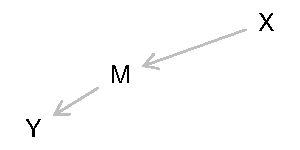
\includegraphics{causality_files/figure-beamer/unnamed-chunk-3-1.pdf}

\end{frame}

\begin{frame}{Potential outcomes: heterogeneous effects}

\textbf{Question}: \(\approx\) or \(=\)?

\end{frame}

\section{Estimands and Estimators}\label{estimands-and-estimators}

\begin{frame}{Estimands}

\begin{itemize}
\tightlist
\item
  The estimand is the thing you want to estimate
\item
  If you are estimating something you should be able to say what your
  estimand is
\item
  You are responsible for your estimand. Your estimator will not tell
  you what your estimand is
\item
  Just because you can calculate something does not mean that you have
  an estimand
\item
  You can test a hypothesis without having an estimand
\end{itemize}

\end{frame}

\begin{frame}{Estimands: The Average Treatment Effect}

\begin{itemize}
\item
  The most common estimand is the \textbf{average treatment effect}
\item
  This is a \textbf{summary} of individual treatment effects:
  \[\tau_i = Y_i(1) - Y_i(0)\]
\item
  For persons 1 and 2, the average is:
  \[\tau = \frac{1}{2}(Y_1(1) - Y_1(0)) + \frac{1}{2}(Y_2(1) - Y_2(0))\]
\item
  More generally: \[\tau = \sum_i\frac{1}{n}(Y_i(1) - Y_i(0))\]
\end{itemize}

\end{frame}

\begin{frame}{Estimands: ATE, ATT, ATC, S-, P-, C-, ITT, LATE}

Say that units are randomly assigned to treatment in different strata
(maybe just one); with fixed, though possibly different, shares assigned
in each stratum. Then the key estimands and estimators are: \scriptsize

\begin{table}[htbp] \scriptsize
    \centering
        \begin{tabular}{rlclrl} \scriptsize 
$\label{ATE} \tau_{ATE} \equiv$&$E\left(\tau_i\right) $&$=$&$ \sum\nolimits_{x} \frac{w_x}{\sum\nolimits_{j}w_{j}}\tau_x  $&$ \widehat{\tau}_{ATE} =$&$\sum\nolimits_{x} \frac{w_x}{\sum\nolimits_{j}w_{j}}\widehat{\tau}_x$ \\
$\label{ATT} \tau_{ATT} \equiv$&$E\left(\tau_i\right | Z_i = 1) $&=&$\sum\nolimits_{x} \frac{p_xw_x}{\sum\nolimits_{j}p_jw_j}\tau_x  $&$  \widehat{\tau}_{ATT} =$&$\sum\nolimits_{x} \frac{p_xw_x}{\sum\nolimits_{j}p_jw_j}\widehat{\tau}_x$ \\
$\label{ATC} \tau_{ATC} \equiv$&$E\left(\tau_i\right |  Z_i = 0) $&=&$\sum\nolimits_{x} \frac{(1-p_x)w_x}{\sum\nolimits_{j}(1-p_j)w_j}\tau_x  $&$ \widehat{\tau}_{ATC} =$&$\sum\nolimits_{x} \frac{(1-p_x)w_x}{\sum\nolimits_{j}(1-p_j)w_j}\widehat{\tau}_x $
        \end{tabular}
\end{table}

where \(x\) indexes strata, \(p_x\) is the share of units in each
stratum that is treated, and \(w_x\) is the size of a stratum.

Here:

\begin{itemize}
    \item ATE is Average Treatment Effect (all units)
    \item ATT is Average Treatment Effect on the Treated
    \item ATC is Average Treatment Effect on the Controls
    \end{itemize}

\end{frame}

\begin{frame}{Estimands: ATE, ATT, ATC, S-, P-, C-, ITT, LATE}

\footnotesize
In addition, each of these can be targets of interest:

\begin{itemize} 
    \item for the \textbf{population}, in which case we refer to PATE, PATT, PATC and $\widehat{PATE}, \widehat{PATT},  \widehat{PATC}$
    \item for a \textbf{sample}, in which case we refer to SATE, SATT, SATC, and $\widehat{SATE}, \widehat{SATT},  \widehat{SATC}$
\end{itemize}

And for different subgroups,

\begin{itemize} 
    \item given some value on a covariate, in which case we refer to CATE (conditional average treatment effect)
    \item for unobservable subgroups, we estimate LATE (Local Average Treatment Effect (see below).
\end{itemize}

With non-compliance we might estimate ITT ---the ``intention to treat''
effect

\bigskip
Skip to \hyperlink{Fixer}{\beamergotobutton{Fixer}} or
\hyperlink{nools}{\beamergotobutton{Inference 1}} or
\hyperlink{ideas}{\beamerreturnbutton{Big Ideas}}

\end{frame}

\begin{frame}{Exercise your potential outcomes 1}

Consider the following potential outcomes table:

\begin{table} \centering
\begin{tabular}{c|c|c|c}
Unit    &Y(0)   &Y(1)   &$\tau_i$ \\ \hline
1   & 4 & 3 \\
2   & 2 & 3 \\
3   & 1 & 3 \\
4   & 1 & 3 \\
5   & 2 & 3 
\end{tabular} 
\end{table}

\color{red}\textbf{Questions for us:} What are the unit level treatment
effects? What is the average treatment effect?

\end{frame}

\begin{frame}{Exercise your potential outcomes 2}

Consider the following potential outcomes table:

\begin{table} \centering

    \begin{tabular}{c|c|c}
        In treatment?   &Y(0)   &Y(1)  \\ \hline
        Yes &   & 2 \\
        No  & 3 &   \\
        No  & 1 &   \\
        Yes &   & 3 \\
        Yes &   & 3 \\
        No  & 2 &   
    \end{tabular} 
\end{table}

\color{red}\textbf{Questions for us: } Fill in the blanks.

\begin{itemize}
    \item Assuming a constant treatment effect of $+1$ 
    \item Assuming a constant treatment effect of $-1$ 
    \item Assuming an \textit{average} treatment effect of $0$
\end{itemize}

\color{red} What is the actual treatment effect?

\end{frame}

\section{Endogeneous subgroups}\label{endogeneous-subgroups}

\begin{frame}{Endogeneous Subgroups}

Experiments often give rise to endogenous subgroups. The potential
outcomes framework can make it clear why this can cause problems.

\end{frame}

\begin{frame}{Heterogeneous Effects with Endogeneous Categories}

\begin{itemize} 
\item Problems arise in analyses of subgroups when the categories themselves are affected by treatment
\item Example from our work:
    \begin{itemize}
        \item You want to know if an intervention affects reporting on violence against women
        \item You measure the share of all subjects that experienced violence that file reports
        \item The problem is that which subjects experienced violence is itself a function of treatment
    \end{itemize}
\end{itemize}

\end{frame}

\begin{frame}{Heterogeneous Effects with Endogeneous Categories}

It is possible that in truth no one's reporting behavior has changed,
what has changed is the propensity of people with different propensities
to report to experience violence:

\begin{table} \scriptsize
        \centering
        \begin{tabular}{rcc|cc|cc}
            
            & \multicolumn{ 2}{c}{Violence(Treatment)} & \multicolumn{ 4}{c}{Reporting(Treatment, Violence)} \\
            
            &       V(0) &       V(1) &     R(0,1) &     R(1,1) &     R(0,0) &     R(1,0) \\ \hline
            
            Type 1 (reporter) &          1 &          1 &          1 &          1 &          0 &          0 \\
            
            Type 2 (non reporter) &          1 &          0 &          0 &          0 &          0 &          0 \\          
        \end{tabular}  
    \end{table}

Expected reporting given violence in control = Pr(Type 1)

Expected reporting given violence in treatment = 100\%

\color{red} \textbf{Question}: What is the actual effect of treatment on
the propensity to report violence?

\end{frame}

\begin{frame}{Heterogeneous Effects with Endogeneous Categories}

It is possible that in truth no one's reporting behavior has changed,
what has changed is the propensity of people with different propensities
to report to experience violence:

\begin{table}
\centering
\begin{tabular}{c|cc|cc|c}\scriptsize

           & \multicolumn{ 2}{c}{Reporters} & \multicolumn{ 2}{c}{Non reporters} &            \\ \hline
           & \multicolumn{ 2}{c}{Experience Violence} & \multicolumn{ 2}{c}{Experience Violence} &            \\ \hline \hline
           &         No &        Yes &        No  &        Yes &  \% Report \\

   Control &         25 &         {\color{red}25} &         25 &        {\color{red}25} &       {\color{red} $\frac{25}{25+25}$}= 50\% \\  
   & & & & \\
  Treatment &         25 &         {\color{red}25} &         50 &          {\color{red}0} &      {\color{red}$\frac{25}{25+0}$}=100\% \\ \hline

\end{tabular}  
\end{table}

\end{frame}

\begin{frame}{Heterogeneous Effects with Endogeneous Categories}

This problem can arise as easily in seemingly simple field experiments.
Example:

\begin{itemize}
  \item In one study we provided constituents with information about performance of politicians
  \item we told politicians in advance so that they could take action
  \item we wanted to see whether voters punished poorly performing politicians
  \item what's the problem?
\end{itemize}

\end{frame}

\section{Heterogeneous Effects with Endogeneous
Categories}\label{heterogeneous-effects-with-endogeneous-categories-4}

In such cases you can:

\begin{itemize}
\item Examine the joint distribution of multiple outcomes
\item Condition on pretreatment features only
\item Engage in mediation analysis
\end{itemize}

\end{document}
